   
        
        \begin{ledgroupsized}[r]{120mm}
        \footnotesize 
        \pstart        
        \noindent\textbf{\"{U}berlieferung:}  
        \pend
        \end{ledgroupsized}
      
       
              \begin{ledgroupsized}[r]{114mm}
              \footnotesize 
              \pstart \parindent -6mm
              \makebox[6mm][l]{\textit{L}}Konzept: LH XXXVIII Bl. 158\textendash 161. 2 Bog. 2\textsuperscript{o}. Ca. 7 S. Seiten einspaltig beschrieben, nur Bl. 159 r\textsuperscript{o} untere H\"{a}lfte dreispaltig und Bl. 159 v\textsuperscript{o} zweispaltig beschrieben. Auf Bl. 159 v\textsuperscript{o} ist nur das mittlere Drittel beschrieben, und auf der letzten Seite (161 v\textsuperscript{o}) ist das untere Drittel leer. Die Abfolge der Bl\"{a}tter kann mit Hilfe der Abfolge der exzerpierten Seiten in Witsen und einiger Beobachtungen in Leibniz' Manuskripten rekonstruiert werden. Direkte \"{U}berg\"{a}nge sind feststellbar von 159 r\textsuperscript{o} mittlere Spalte nach 159 v\textsuperscript{o} rechte Spalte, von 159 r\textsuperscript{o} rechte Spalte nach 159 v\textsuperscript{o} linke Spalte, und von 161 r\textsuperscript{o} nach 161 v\textsuperscript{o}. Bl. 160 v\textsuperscript{o} bricht im Satz ab, m\"{o}glicherweise ist der Text nicht vollst\"{a}ndig. Aus diesen Beobachtungen ergibt sich als Reihenfolge 158 r\textsuperscript{o}, 158 v\textsuperscript{o}, 159 r\textsuperscript{o} obere H\"{a}lfte, unten linke Sp., mittlere Sp., 159 v\textsuperscript{o} rechte Sp., 159 r\textsuperscript{o} rechte Sp., 159 v\textsuperscript{o} linke Sp., 161 r\textsuperscript{o}, 161 v\textsuperscript{o}, 160 r\textsuperscript{o} und 160 v\textsuperscript{o}.\\Cc 2, Nr. 1558 A, B \pend
              \end{ledgroupsized}
        %\normalsize
        \vspace*{5mm}
        \begin{ledgroup}
        \footnotesize 
        \pstart
      \noindent\footnotesize{\textbf{Datierungsgr\"{u}nde}: Trotz einiger Hinweise auf eine Besch\"{a}ftigung Leibniz' mit Witsens Buch (\textit{LSB} IV, 4 N. 6; III, 4 N. 23; I, 18 N. 222; LH XXXVIII, Bl. 104~r\textsuperscript{o}) ist daraus der Zeitpunkt der Rezeption des Buches durch Leibniz  nicht zu ermitteln. Weil Witsen sich beim holl\"{a}n\-disch-spanischen Heer befand, kann eine Begegnung zwischen ihm und Leibniz w\"{a}hrend dessen Aufenthalt in Amsterdam November 1676 ausgeschlossen werden, womit der auff\"{a}lligste Grund f\"{u}r eine Datierung in diese Zeit entf\"{a}llt. Daher muss zur Datierung auf den Texttr\"{a}ger zur\"{u}ckgegriffen werden. Die Kennzeichen des Texttr\"{a}gers sind Pariser Papier und ein Wasserzeichen in beiden B\"{o}gen, das unterschiedlich auf 1674 oder 1676 datiert wird. Damit ist ein Hinweis auf Anfertigung dieser Exzerpte w\"{a}hrend des Aufenthaltes in Paris gegeben. Das exzerpierte Werk des Nicolaes Witsen, \cite{00153}\textit{Scheeps-Bouw en Bestier}, wurde bereits April 1671 in einem Brief an Leibniz erw\"{a}hnt (\textit{LSB} I, 1 N. 83). Ebenfalls ist das Buch in dem von Leibniz intensiv rezipierten \textit{JS} besprochen worden (\cite{00274}\textit{JS} 4 (1675), S.~173\textendash 175). Der Text wirkt trotz einiger unzusammen\-h\"{a}ngender \"{U}berg\"{a}nge weitgehend homogen, so dass eine Entstehung in mehreren, auseinander liegenden Phasen unwahrscheinlich ist. Nach Abw\"{a}gung dieser Beobachtungen ist das St\"{u}ck aufgrund des Texttr\"{a}gers in die Pariser Zeit zu datieren. Wegen des Wasserzeichens und des Artikels im \textit{JS} erfolgt eine weitere Eingrenzung auf die Jahre 1675 und 1676.}
        \pend
        \end{ledgroup}
      
        \newpage
        \pstart 
        \normalsize
      [158 r\textsuperscript{o}] \edtext{\textit{Scheeps}\edlabel{scheepsstart}}{{\xxref{scheepsstart}{scheepsend}}\lemma{\textit{Scheeps}}\Bfootnote{Von \textit{Scheeps Bow} bis et fecit vgl. \textsc{N. Witsen}, \cite{00153}\textit{Scheeps-Bouw}, Amsterdam 1671, Titelkupfer.}} \textit{Bow en Bestier dor N. Witsen}\protect\index{Namensregister}{\textso{Witsen,} Nicolaes 1641\textendash 1717}. Romain \textit{de Hooghe}\protect\index{Namensregister}{\textso{Hooghe,} Romeyn de 1645\textendash 1708} inv. et fecit\edlabel{scheepsend}.
      \pend 
      \pstart \edtext{\textit{Aeloude\edlabel{aeloudestart}}}{{\xxref{aeloudestart}{aeloudeend}}\lemma{\textit{Aeloude}}\Bfootnote{Von Aeloude bis 1671 fol. vgl. \textsc{N. Witsen}, \cite{00153}a.a.O., Titelseite.}} \textit{en hedendaegsche Scheeps}-\edtext{\textit{bouw}}{\lemma{Scheeps-}\Afootnote{ \textit{ (1) }\ bow \textit{ (2) }\ \textit{bouw} \textit{ L}}} \textit{en bestier, Waerin wiitloopigh wert verhandelt} \edtext{\textit{de wiize}}{\lemma{\textit{de}}\Afootnote{ \textit{ (1) }\ wise \textit{ (2) }\ wiize \textit{ L}}} \textit{van scheeps-timmern by} \edtext{\textit{Grieken}}{\lemma{\textit{by}}\Afootnote{ \textit{ (1) }\ Griecken \textit{ (2) }\ \textit{Grieken} \textit{ L}}} \textit{en Romeynen: scheeps}-oefningen,\textit{ striiden, tucht, straffe, wetten en gewoonten}. Benevens \textit{Evenmaetige grootheden van schepen onses tijts ontleet in alle hare deelen, verschil van bowen tusschen uitheemschen en onzen landaert: indisch Vaertuygh, Galey-bow, hedendaegsche Scheepsplichten, verrijckt met een reex verclaerde Zeemans-spreeckwoorden en benamingen, beschreven door Nicolaes Witsen}\protect\index{Namensregister}{\textso{Witsen,} Nicolaes 1641\textendash 1717}[.] \textit{t' Amsterdam}\protect\index{Ortsregister}{Amsterdam} \textit{by Casparus Commelijn}\protect\index{Namensregister}{\textso{Commelijn,} Caspar 1634\textendash 1693}\textit{; Broer}\protect\index{Namensregister}{\textso{Appelaer,} Broer, Amsterdamer Buchdrucker, belegt 1674?\textendash 1684} \textit{en Jan Appelaer}\protect\index{Namensregister}{\textso{Appelaer,} Jan, Amsterdamer Buchdrucker, belegt 1643\textendash 1687} Book \textit{verkoopers Anno 1671 fol.\edlabel{aeloudeend}}
      \pend
       \pstart 
\textit{Il}\edlabel{commendatorestart} \edtext{\textit{Commendatore}}{{\xxref{commendatorestart}{commendatoreend}}\lemma{Commendatore}\Bfootnote{Von Il Commendatore bis collectanea vgl. \textsc{N. Witsen}, \cite{00153}a.a.O., S. II der Einleitung.}} \edtext{\textit{Carlo Antonio dal}}{\lemma{\textit{Antonio}}\Afootnote{ \textit{ (1) }\ del \textit{ (2) }\ \textit{dal} \textit{ L}}} \textit{Pozzo}\protect\index{Namensregister}{\textso{Pozzo di Borgo,} Carlo Antonio 1633\textendash 1687}, Eques Romanus \edtext{autori misit}{\lemma{Romanus}\Afootnote{ \textit{ (1) }\ hat den \textit{ (2) }\ autori misit \textit{ L}}} veteres navium figuras ex marmoribus et nummis. Item collectanea Pyrrhi Ligorii\protect\index{Namensregister}{\textso{Ligorio} (Ligorius), Pirro 1514\textendash 1583} Equitis Neapolitani collectanea\edlabel{commendatoreend}.
\pend 
\pstart \edtext{Tjassens Scheepbestier \textit{of politie}\protect\index{Namensregister}{\textso{Tjassens,} Johan ?\textendash 1670}}{\lemma{\textit{Tjassens}}\Bfootnote{Von Tjassens bis politie vgl. \textsc{N. Witsen}, \cite{00153}a.a.O., S. III der Einleitung.}}\edtext{}{\lemma{\textit{politie}}\Bfootnote{\textsc{J. Tjassens}, \cite{00227}\textit{Zee-Politie der vereenichde Nederlanden}, 's-Graven-Hage 1670.}} 
\pend 
\pstart \edtext{Sheeps\edlabel{bartholomaeistart}}{{\xxref{bartholomaeistart}{bartholomaeiend}}\lemma{Sheeps}\Bfootnote{Von Sheeps bis Fronsperger vgl. \textsc{N. Witsen}, \cite{00153}a.a.O., S. IV der  Einleitung.}} timmering Bartholomaei \edtext{Crescentii}{\lemma{Crescentii}\Bfootnote{\textsc{B. Crescentio}, \cite{00232}\textit{Nautica Mediterranea}, Rom 1602.}}\protect\index{Namensregister}{\textso{Crescenzio} (Crescentius), Bartolomeo, erw\"{a}hnt 1591\textendash 1601}. Romani Invenitur et liber Italicus satis grandis hoc habet. \textit{Del vera et reale arte della navigatione del governo e disciplina del mare, et di le combattere in armate esquadrone}, Romae\protect\index{Ortsregister}{Rom (Roma)} editus. Et alius Florentiae\protect\index{Ortsregister}{Florenz (Fiorenze, Florentia)} cui tit. \textit{l'Architettura nautica divascelli} etc.\edtext{}{\lemma{etc.}\Bfootnote{\textsc{R. Dudley}, \cite{00226}\textit{Dell'arcano del mare}, Florenz 1661.}}
\pend 
\clearpage 
\pstart De Gallicarum navium\protect\index{Sachverzeichnis}{navis} structura et regimine P. Fournier\protect\index{Namensregister}{\textso{Fournier} (Fournerius), Georges SJ 1595\textendash 1652}, item Hobier\protect\index{Namensregister}{\textso{Hobier,} Ithier ?\textendash 1644?}; in Germanico, Jos. Furtenbach\protect\index{Namensregister}{\textso{Furttenbach} (Furtenbach), Joseph 1591\textendash 1667}, et Leond. Fronsperger\protect\index{Namensregister}{\textso{Fronsperger,} Leonhart 1520?\textendash 1575}\edlabel{bartholomaeiend}. \edtext{Dicit\edlabel{dicitstart}}{{\xxref{dicitstart}{dicitend}}\lemma{Dicit}\Bfootnote{Von Dicit bis adibant vgl. \textsc{N. Witsen}, \cite{00153}a.a.O., S. V der Einleitung.}} nullas hodie cartas arcanas esse, indici\protect\index{Ortsregister}{Indien (India)} itineris, omnia nota Batavis\protect\index{Ortsregister}{Holland (Hollandia)} et aliis sciri, nec tamen posse alios eos imitari. Olim Groenlandiam\protect\index{Ortsregister}{Gronland@Gr\"{o}nland (Groenlandia)} tantum Biscaini adibant\edlabel{dicitend}. \edtext{Ait\edlabel{delineationesstart}}{{\xxref{delineationesstart}{delineationesend}}\lemma{Ait}\Bfootnote{Von Ait bis delineationes vgl. \textsc{N. Witsen}, \cite{00153}a.a.O., S. VI der Einleitung.}} \edtext{apud}{\lemma{}\Afootnote{apud \textit{ erg.} \textit{ L}}} patrem suum Cornel. Witsen\protect\index{Namensregister}{\textso{Witsen,} Cornelis 1605\textendash 1669} se reperisse multas figurarum Nauticarum delineationes\edlabel{delineationesend}. \edtext{Adjecti\edlabel{adjectistart}}{{\xxref{adjectistart}{adjectiend}}\lemma{Adjecti}\Bfootnote{Von Adjecti bis Amstelodamensis vgl. \textsc{N. Witsen}, \cite{00153}a.a.O., Widmung und Elegia.}} versus Sam. Tennullii\protect\index{Namensregister}{\textso{Nuyl} (Tennullius), Samuel ten 1635\textendash 1688} professoris Universitatis Noviomagensis Witsen\protect\index{Namensregister}{\textso{Witsen,} Nicolaes 1641\textendash 1717} J.U.D. et senator \textit{Amstelodamensis}\edlabel{adjectiend}.
\pend
\pstart \edtext{M.\edlabel{meibomiusstart} Meibomius\protect\index{Namensregister}{\textso{Meibom} (Meibomius), Marcus 1630\textendash 1711}}{{\xxref{meibomiusstart}{meibomiusend}}\lemma{M. Mei\-bomius}\Bfootnote{Von M. Meibomius bis Meybomium vgl. \textsc{N. Witsen}, \cite{00153}a.a.O., S.~13.}} ad Vitruvium \edtext{Jac.}{\lemma{}\Afootnote{Jac. \textit{ erg.} \textit{ L}}} Palmerius\protect\index{Namensregister}{\textso{Le Paulmier de Grentemesnil,} Jacques 1587\textendash 1670} \textit{ad Memnonis fragmentum} \edtext{de triremibus}{\lemma{de}\Afootnote{ \textit{ (1) }\ re nautica \textit{ (2) }\ triremibus \textit{ L}}} videri possunt. Palmerius\protect\index{Namensregister}{\textso{Le Paulmier de Grentemesnil,} Jacques 1587\textendash 1670} sequitur Meybomium\protect\index{Namensregister}{\textso{Meibom} (Meibomius), Marcus 1630\textendash 1711}\edlabel{meibomiusend}.
\pend 
\pstart \textso{pag. 47}. \edtext{\textit{ziet}\edlabel{zietstart}}{{\xxref{zietstart}{zietend}}\lemma{\textit{ziet}}\Bfootnote{Von ziet bis typographus vgl. \textsc{N. Witsen}, \cite{00153}a.a.O., S.~47.}} \textit{by Wechelus}\protect\index{Namensregister}{\textso{Wechel} (Wechelus), Andreas 1510\textendash 1581} \edtext{\textit{in zijn boek}}{\lemma{\textit{boek}}\Bfootnote{Vermutl. die durch J. Bongars\protect\index{Namensregister}{\textso{Bongars} (Bongartius), Jacques 1554\textendash 1612} besorgte und durch A. Wechels\protect\index{Namensregister}{\textso{Wechel} (Wechelus), Andreas 1510\textendash 1581} Erben verlegte Ausgabe des \textsc{Guibert de Nogent}, \cite{00228}\textit{Gesta Dei per Francos}, Hannover 1611. Vgl. auch den durch Witsen hier und S. 85 erw\"{a}hnten Sanuto\protect\index{Namensregister}{\textso{Sanuto,} Marino 1466\textendash 1535} und dessen Beschreibung des Schiffbaus zur Zeit der Kreuzz\"{u}ge, \cite{00233}\textsc{M. Sanuto}, \textit{Liber secretorum fidelium crucis}, (= \textit{Primum in Bongartii opere Gesta Dei per Francos} intitulato ed.), Hannover 1611.}} \textit{Gesta DEI per francos}, cum \edtext{sit tantum}{\lemma{sit}\Afootnote{ \textit{ (1) }\ liber \textit{ (2) }\ tantum \textit{ L}}} typographus\edlabel{zietend}.
\pend 
\pstart \textso{pag. 141} \edtext{habet\edlabel{habetstart}}{{\xxref{habetstart}{habetend}}\lemma{habet}\Bfootnote{Von habet bis impelletur in de vgl. \textsc{N. Witsen}, \cite{00153}a.a.O., S.~141.}} propositiones quasdam de navium\protect\index{Sachverzeichnis}{navis} \edtext{motu, et velis ubi}{\lemma{navium}\Afootnote{ \textit{ (1) }\ situ, ubi \textit{ (2) }\ motu, et velis ubi \textit{ L}}} supponit, ventum agere in linea non obliquitatis suae, sed ad velum\protect\index{Sachverzeichnis}{velum} perpendiculari, ut 
%zeitz auskommentiert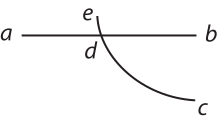
\includegraphics[width=0.2\textwidth]{images/38_158r1}
 ut \textit{ab} velum \textit{cd} ventus, navis\protect\index{Sachverzeichnis}{navis} impelletur in \textit{de}\edlabel{habetend}.\pend 
\pstart \textso{Witsen}\protect\index{Namensregister}{\textso{Witsen,} Nicolaes 1641\textendash 1717} \textso{Nautic. p. 1. pag. 177} \textit{tweegekielt}\edlabel{tweegekieltstart} schip\protect\index{Sachverzeichnis}{Schiff!tweegekielt}\edtext{}{{\xxref{tweegekieltstart}{tweegekieltend}}\lemma{\textso{pag. 177}}\Bfootnote{Von tweegekielt bis vermeerdern vgl. \textsc{N. Witsen}, \cite{00153}a.a.O., S.~177.}}, \textit{nevens andere} ungemeene \textit{Scheeps}\protect\index{Sachverzeichnis}{schip} gebowen. \textendash\ Il n' y a pas long temps, dit il, qu' on a mis \`{a} Londres\protect\index{Ortsregister}{London (Londinum)} un vaisseau\protect\index{Sachverzeichnis}{vaisseau}\edtext{}{\lemma{}\Afootnote{vaisseau \textbar\ entier \textit{ gestr.}\ \textbar\ en \textit{ L}}} en mer, qui estoit a double fonds. Sans ballast ou lest, il entroit dans l'eau \`{a} 7 $\displaystyle\frac{1}{2}$\rule[-4mm]{0mm}{10mm} pieds. Et voila la construction. On bastissoit deux petits vaisseaux\protect\index{Sachverzeichnis}{vaisseau}, leur (\textit{Kielen}\protect\index{Sachverzeichnis}{Kiel}) fonds sur l'eau, et \edtext{[joints]\edtext{}{\Afootnote{jointes\textit{\ L \"{a}ndert Hrsg. } }} l'un \`{a} l'autre par}{\lemma{et}\Afootnote{ \textit{ (1) }\ par \textit{ (2) }\ [joints] l'un \`{a} l'autre par \textit{ L}}} le bord chaque fonds de 80 pieds. Le vaisseau\protect\index{Sachverzeichnis}{vaisseau} tout entier 32 pieds de largeur, 14 de creux ou de profondeur. Il portoit 50 pieces de canon, 300\edtext{}{\lemma{300 hommes}\Bfootnote{Bei Witsen: 200 man}} hommes, et des provisions pour trois mois, of wanneer last droeg 50 Engelsche tonnen. Il estoit bon voilier, dont les raisons estoit, la multitude des voiles\protect\index{Sachverzeichnis}{voile}, et la legeret\'{e} du bastiment. L'eau passant entre deux fonds \textit{weerhielt hem van het afdrijven en omslaen. De Kiel}\protect\index{Sachverzeichnis}{Kiel} \textit{was met uistekende houten}\protect\index{Sachverzeichnis}{hout} \edtext{\textit{voorzien}}{\lemma{\textit{houten}}\Afootnote{ \textit{ (1) }\ voortien \textit{ (2) }\ \textit{voorzien} \textit{ L}}}, \textit{die het} ship\protect\index{Sachverzeichnis}{schip} \textit{voor} stooten \textit{tegen te grond behoeden. Geen Schip\protect\index{Sachverzeichnis}{schip} luisterte} zo \textit{wel} nae zyn \textit{roer}\protect\index{Sachverzeichnis}{roer} \textit{als dit, en} zulcks \textit{om dat het water, t'geen tusschen} beede \textit{doorgong, het roer\protect\index{Sachverzeichnis}{roer} sloeg met een zer grooten drifft en vaert. Het Schip\protect\index{Sachverzeichnis}{schip} was kantig en niet} rond \textit{van beloop}, waeromb \textit{by de} bowers \edtext{\textit{geoordeelt wiert}}{\lemma{\textit{geoordeelt}}\Afootnote{ \textit{ (1) }\ wird \textit{ (2) }\ \textit{wiert} \textit{ L}}}, \textit{dat het vaster op't water most leggen als} andre \edtext{\textit{Schepen}}{\lemma{andre}\Afootnote{ \textit{ (1) }\ Scheepen \textit{ (2) }\ \textit{Schepen} \textit{ L}}}, \textit{en by gevolg zijn onderste} shut \textit{by quaet weder zo wel} gebruicken, \textit{als het bovenste. Binnewaerts tusschen} \edtext{\textit{beide}}{\lemma{tusschen}\Afootnote{ \textit{ (1) }\ beyde \textit{ (2) }\ \textit{beide} \textit{ L}}} Kielen\protect\index{Sachverzeichnis}{Kiel} \textit{in, kon men by stilte zoo wel roeien als buitewaerts, t'geen} en \textit{snellen loop aen het Schip}\protect\index{Sachverzeichnis}{schip} veroorsaekte.
\pend 
\pstart \textit{Aen} dese fond schiint \textit{niet} ongeliik \textit{te} zyn \textit{dat Schip\protect\index{Sachverzeichnis}{schip} t'welck twee voorsteevens\protect\index{Sachverzeichnis}{vorsteven} hadde, waer tusschen zeker wercktuig in t'water} nader \textit{liet, 't geen by twee mannen op het Schip\protect\index{Sachverzeichnis}{schip} staende wiert omgedraeit, waer mede de vaert wierd} \edtext{\textit{vertraegt}}{\lemma{\textit{wierd}}\Afootnote{ \textit{ (1) }\ omged \textit{ (2) }\ \textit{vertraegt} \textit{ L}}} \textit{of verhaest}.
\pend 
\pstart \textit{Indien men schepen\protect\index{Sachverzeichnis}{schip} wilde maken die zonder} lossen \textit{van hunnen last over droogtens en ondiepten konnen varen} zo \textit{maekt men en dubbelden boden daer men lederne zacken tusschen brengt, die met blaes-balken\protect\index{Sachverzeichnis}{blaasbalg} opgeblazen konnen werden. Wanneer dan} dese \textit{zacken} voll \textit{wind zullen zijn, dan zal het Schip}\protect\index{Sachverzeichnis}{schip} \edtext{riizen}{\lemma{\textit{Schip}}\Afootnote{ \textit{ (1) }\ zijsen \textit{ (2) }\ riizen \textit{ L}}} \textit{en driftiger werden als voor heen}.
\pend 
\clearpage 
\pstart \textit{Met scheppers zoude men op veelerleie} wiise \textit{schepen\protect\index{Sachverzeichnis}{schip} konnen toestellen, die by een of meer mannen bewogen konnen werden}, welk \textit{traag of} \edtext{\textit{snel}}{\lemma{\textit{of}}\Afootnote{ \textit{ (1) }\ snell \textit{ (2) }\ \textit{snel} \textit{ L}}} \textit{voort zoude gaen na het} \edtext{\textit{getal}}{\lemma{\textit{het}}\Afootnote{ \textit{ (1) }\ getae \textit{ (2) }\ \textit{getal} \textit{ L}}} \textit{van de raderen, en de macht die daer aen wierde gestelt}. 
\pend 
\pstart \textit{By zeckre Jesuit in Duitslant\protect\index{Ortsregister}{
Deutschland (Germania, Duitsland)} is ervonden een zeil\protect\index{Sachverzeichnis}{zeil} 't geen} geliik \textit{een molen om een mast\protect\index{Sachverzeichnis}{mast} of spil\protect\index{Sachverzeichnis}{spil} die op het ship\protect\index{Sachverzeichnis}{schip} staet, van de} wind \textit{gedraeit} worden, \textit{deze spil\protect\index{Sachverzeichnis}{spil} beweegt onder eenige sheppers, of riemen} \edtext{(remos movet ventus)}{\lemma{}\Afootnote{(remos movet ventus) \textit{ erg.} \textit{ L}}}, \textit{die het schip\protect\index{Sachverzeichnis}{schip} sijn voortganck}\protect\index{Sachverzeichnis}{schip\textendash voortgang} toen \textit{hebben. Het zeil\protect\index{Sachverzeichnis}{zeil} bestaet in 3 of 4 vlercken, die om den spil\protect\index{Sachverzeichnis}{schip} voornoemt konnen werden gedraeit, hoe het waeyen van de wint oock moge} zyn. \textit{Het stellen van deze raederen\protect\index{Sachverzeichnis}{rad}, en hoe men den loop vertragen (retardare) of verhaesten kan, met de tanden van het rat te verminderen of vermeerdern}\edlabel{tweegekieltend}, \edtext{gelieft\edlabel{gelieftstart}}{{\xxref{gelieftstart}{gelieftend}}\lemma{gelieft}\Bfootnote{Von gelieft bis gestooken vgl. \textsc{N. Witsen}, \cite{00153}a.a.O., S.~178.}} volmaeckteliik te zijn hy de \textit{vermaerden Schottus}\protect\index{Namensregister}{\textso{Schott} (Schottus), Caspar SJ 1608\textendash 1666}. 
\pend 
\pstart Vanum esse videtur, quod Drebel\protect\index{Namensregister}{\textso{Drebbel} (Drebelius, Drebel), Cornelius 1572\textendash 1633} et Mersennus\protect\index{Namensregister}{\textso{Mersenne} (Mersennus), Marin 1588\textendash 1648} dixere posse sub aqua navigari hausto aere per natatiles in summo tubos coriaceos\protect\index{Sachverzeichnis}{tubus!coriaceus}.
\pend 
\pstart Navis Melitensis\protect\index{Sachverzeichnis}{navis!Melitensis} rotis\protect\index{Sachverzeichnis}{rota} acta, et hominum vi\protect\index{Sachverzeichnis}{vis!hominis}, et, Roterodamensis\protect\index{Sachverzeichnis}{navis!Roterodamensis}, inutiles fuere. \textit{Op}'t he \textit{Rhosne men shepen}\protect\index{Sachverzeichnis}{schip} \edtext{\textit{vint}}{\lemma{\textit{shepen}}\Afootnote{ \textit{ (1) }\ \textit{vind} \textit{ (2) }\ \textit{vint} \textit{ L}}}\textit{, waer een sleuf onder midden doorgaet, die door-togtaen t'water geeft; welk water een} rad\protect\index{Sachverzeichnis}{rad} \textit{om} driift, \textit{t' geen boven aen een spil}\protect\index{Sachverzeichnis}{spil} \textit{een} \edtext{\textit{touw}}{\lemma{\textit{een}}\Afootnote{ \textit{ (1) }\ \textit{tow} \textit{ (2) }\ \textit{touw} \textit{ L}}} \textit{opwint, welck touw een stuck-weegs voor} uyt \textit{aen lant vast is, en dus moet het Schip}\protect\index{Sachverzeichnis}{schip} nootwendig \textit{tegen stroom op voortgaen, zoo lang, tot dat het} tow \textit{geheel om de spil\protect\index{Sachverzeichnis}{spil} gewonden is, als wanneer men het zelvige weder los} \edtext{\textit{maeckt}}{\lemma{\textit{los}}\Afootnote{ \textit{ (1) }\ \textit{maekt} \textit{ (2) }\ \textit{maeckt} \textit{ L}}} \textit{en voor} uyt \textit{brengt, op dat het weder om de spil\protect\index{Sachverzeichnis}{spil} gewonden werde, en het Schip\protect\index{Sachverzeichnis}{schip} zoo doe vortgaen}.
\pend 
\pstart Bessonius\protect\index{Namensregister}{\textso{Besson} (Bessonius), Jacques 1510\textendash 1576} exemplo Vitruvii\protect\index{Namensregister}{\textso{Vitruvius Pollio,} Marcus ca. 70\textendash 10 v. Chr.} navim\protect\index{Sachverzeichnis}{navis} delineavit, quae iter percursum sine ulla nota externa. Scilicet in navis\protect\index{Sachverzeichnis}{navis} jam apertura, qua intrans aqua agit rotas\protect\index{Sachverzeichnis}{rota} \edtext{indici}{\lemma{rotas}\Afootnote{ \textit{ (1) }\ ad \textit{ (2) }\ indici \textit{ L}}} applicatas.
\pend 
\pstart Utilis est \edtext{\textit{het Amsterdamsche Modder-molen schip}}{\lemma{est}\Afootnote{ \textit{ (1) }\ navis Amstelodamensis \textit{ (2) }\ \textit{het Amsterdamsche Modder-molen schip} \textit{ L}}}, quod quotidie 50 usque ad 60 schuyten \textit{vol} dreck (+ bove modder +) ex fundo effert, unius equi potentia. Desen \textit{toestel bestaet in een zwaer radt}, benevens \textit{eenige Scheppers, die den modder vatten, boven brengen, en} uytwerpen. \textit{De Scheppers leggen in een sleuf, zoo dat de modder niet spillen en kan. Daer de gronden hart} zyn, \textit{moeten the sheppers scherp} rontaghtig \textit{en van eizer}\protect\index{Sachverzeichnis}{ijzer} zyn: gelijk men ze \textit{tot Dordregt\protect\index{Ortsregister}{Dordrecht} en Rotterdam\protect\index{Ortsregister}{Rotterdam}} gebruyckt. In Nort Holland\protect\index{Ortsregister}{Nordholland (Nort Holland)} \textit{ziet men platachtige vaertuigen, daer zant en steenen mede van de gront boven werden gehaelt 8 of 10 mannen winden daer in een spil\protect\index{Sachverzeichnis}{spil} om, welke} dor \textit{zeker} eiser\protect\index{Sachverzeichnis}{ijzer} \textit{werktuig het} sand \textit{en de steenen} uyt \textit{het water en in het ship\protect\index{Sachverzeichnis}{schip} doen komen}. Ysschuyten\protect\index{Sachverzeichnis}{Ysschuiten} in Holland\protect\index{Ortsregister}{Holland (Hollandia)}, quae velo aguntur, citiusque eunt equo celerrimo ne cadant, \textit{werden planken dwers onder den bodem door \edlabel{gelieftend}gestooken}.
\pend 